% Emacs, this is -*-latex-*-

\title{The JPEG2000 standard (ISO/IEC 15444-1)}
\author{Vicente González Ruiz}
\maketitle
\tableofcontents

\section{JPEG 2000 features~\cite{rabbani2009jpeg}}
\begin{enumerate}
\item Improved compression efficiency (compared to JPEG).
\item Lossy to lossless compression.
\item Multiple resolution representation.
\item Progressive (quality) decoding.
\item Tiling.
\item Region-of-interest (ROI) coding.
\item Error resilience.
\item Random code-stream access and processing.
\end{enumerate}

\section{Intro~\cite{2002.taubman}}
\begin{itemize}
\item \textbf{Lossy \& lossless:} The lossy path has a better RD curve
  than the lossless path.
  \begin{center}
    \svg{graphics/arquitectura_J2K}{600}
  \end{center}
\item \textbf{Quality scalability:} More decoded data, more quality.
  \begin{center}
    \png{graphics/lena_01_jp2}{512}
    \png{graphics/lena_02_jp2}{512}
    \png{graphics/lena_05_jp2}{512}
  \end{center}
  
\item \textbf{Spatial scalability:} More decoded data, more
  resolution.
  \begin{center}
    \resizebox{0.9\textwidth}{!}{
      \begin{tabular}{ccc}
        \png{graphics/lena_128x128_rgb}{512} & 
        \png{graphics/lena_256x256_rgb}{512} & 
        \png{graphics/lena_512x512_rgb}{512}
      \end{tabular}
    }
  \end{center}

\item \textbf{ROI (Regions Of Interest) scalability:}
  \begin{center}
    \png{graphics/lena_512x512_rgb_jp2_roi}{512}
  \end{center}

\end{itemize}

\begin{comment}
\section{>Qu'e es la codificaci'on progresiva?}
\begin{itemize}
\item Debido a la gran cantidad de datos que se generan, la
  transmisi'on de las im'agenes, incluso en un formato comprimido,
  necesitan un cierto tiempo. Cuando es posible reconstruir la imagen
  en el receptor con un sub-conjunto del stream de datos comprimidos,
  hablaremos de codificaci'on progresiva de im'agenes.
  \vspace{-1ex}
  \begin{center}
    \svg{graphics/rate-distortion}{600}
  \end{center}
\end{itemize}
\end{comment}

\section{The JPEG2000 algorithm}
\begin{center}
  \svg{graphics/J2K}{1400}
\end{center}
\begin{enumerate}
\item Color component DC level offset (optional).
\item Intercomponent decorrelation (optional).
\item Spatial decorrelation (2D-DWT).
\item Quantization (only in the lossy path).
\item ROI definition.
\item Entropy coding (tier-1 coding).
\item Bit-stream organization (tier-2 coding).
\end{enumerate}

\section{DC level offset (step 1/6)}
\begin{itemize}
\item [] Depends on the selected path. For each component:
\begin{enumerate}
\item \textbf{Irreversible:} normalize the samples
  $s[{\mbox{\boldmath$n$}}]$ in order to satisfy that
  \begin{equation}
    -\frac{1}{2}\le s[{\mbox{\boldmath$n$}}] \le \frac{1}{2},
  \end{equation}
  where $s[{\mbox{\boldmath$n$}}]=s[x,y]$ is a point.
\item \textbf{Reversible:} substract an offset to 
  $s[{\mbox{\boldmath$n$}}]$ if they does not verify than
  \begin{equation}
    -2^{B-1}\le s[{\mbox{\boldmath$n$}}] < 2^{B-1},
  \end{equation}
  where $B$ is the number of bits/component.
\end{enumerate}
\end{itemize}

\section{Component decorrelation (step 2/6)}
\begin{itemize}
\item [] Only to color (RGB) images.
  \begin{enumerate}
  \item \textbf{Irreversible path:}
    \begin{equation}
      \begin{array}{l}
        \text{Y} = 0.299\text{R}+0.587\text{G}+0.144\text{B}\\
        ~\\
        \text{Cb} = \frac{\displaystyle0.5}{\displaystyle1-0.144}(\text{B}-\text{Y})\\
        ~\\
        \text{Cr} = \frac{\displaystyle0.5}{\displaystyle1-0.299}(\text{R}-\text{Y})
      \end{array}
    \end{equation}
  \item \textbf{Reversible path:}
    \begin{equation}
      \begin{array}{l}
        \text{Y\'{}} =
        \Big\lfloor\frac{\displaystyle\text{R}+2\text{G}+\text{B}}{\displaystyle 4}\Big\rfloor\\
         ~\\
       \text{Db} = \text{B}-\text{G}\\
        ~\\
        \text{Dr} = \text{R}-\text{G}
      \end{array}
    \end{equation}
  \end{enumerate}
\end{itemize}

\section{The 2D DWT (step 3/6)}
\begin{itemize}
\item In JPEG 2000, the 2D DWT is applied independently to each component.
  \begin{enumerate}
  \item \textbf{Irreversible path:}
    \begin{equation}
      \begin{array}{c}
        \begin{array}{ll}
          \multicolumn{2}{l}{L(z) =} \\
          & 0.602949018236\\
          + & 0.266764118443(z^1+z^{-1})\\
          - & 0.078223266529(z^2+z^{-2})\\
          - & 0.016864118443(z^3+z^{-3})\\
          + & 0.026748757411(z^4+z^{-4})
        \end{array}
        \\
        \\
        \begin{array}{ll}
          \multicolumn{2}{l}{H(z) =} \\
          & 0.557543526229\\
          + & 0.295635881557(z^1+z^{-1})\\
          - & 0.028771763114(z^2+z^{-2})\\
          - & 0.045635881557(z^3+z^{-3})
        \end{array}
      \end{array}
      \tag{CDF 9/7}
    \end{equation}
    \newpage
  \item \textbf{Reversible path:}
    \begin{equation}
      \begin{array}{l}
      H(z) = -\frac{1}{8}(z^2+z^{-2}) + \frac{1}{4}(z^1+z^{-1}) +
      \frac{3}{4}\\~\\
      L(z) = -\frac{1}{2}(z^1+z^{-1}) + 1
    \end{array}
    \tag{Spline 5/3}
    \end{equation}
  \end{enumerate}
\end{itemize}

\section{Quantization (step 4/6)}
\subsection*{Irreversible path}  
\begin{equation}
  q_b = \text{sign}(y_b)\Big\lfloor\frac{\displaystyle
    |y_b|}{\displaystyle \Delta_b}\Big\rfloor
\tag{J2KQuant}
\end{equation}
where $q_b$ is the quantized coefficient, $y_b\in [-0.5,0.5]$ is a
wavelet coefficient in the subband $b$ and $\Delta_b$ is the quantizer
step size for the subband $b$, whose value depends on $y_b$ as it is
shown in the next figure (deathzone scalar quantizer):

\begin{center}
  % \resizebox{0.8\textwidth}{!}{\input{../figs/EDQ}}
  % \texfigure{0.8\textwidth}{!}{../figs/EDQ}
  \svg{EDQ}{800}
\end{center}

\begin{comment}
  \item \textbf{Irreversible:} tiene como entrada los coeficientes
    wavelet que est'an en el rango $[-0.5,0.5]$ y como salida una
    palabra binaria (o 'indice de cuantificaci'on) de $x$ bits que
    depende del nivel de compresi'on seleccionado. Esta consiste en
    \begin{equation}
      q_b = \text{sign}(y_b)\Big\lfloor\frac{\displaystyle
        |y_b|}{\displaystyle \Delta_b}\Big\rfloor
    \end{equation}
    donde $y_b$ es un coeficiente wavelet de la banda de frecuencia
    $b$ y $\Delta_b$ es el tama~no del paso del cuantificador escalar
    progresivo con ``deadzone'', es decir, el par'ametro que define el
    nivel de compresi'on. $\Delta_b$ es distinto para cada banda porque
    el peso relativo de cada una de ellas es diferente (v'ease la
    Secci'on \ref{sec:pesos_bandas}).

    Un ejemplo para dos primeros niveles de cuantificaci'on diferentes:
    \begin{center}
      %\resizebox{0.8\textwidth}{!}{\input{../figs/EDQ}}
      %\texfigure{0.8\textwidth}{!}{../figs/EDQ}
      \svg{EDQ}{600}
    \end{center}

    Los coeficientes cuantificados ('indices de cuantificaci'on) $q_b$
    son los que se codifican entr'opicamente.
\end{comment}

\subsection*{Reversible path}
There is no quantization:
\begin{equation}
  q_b = y_b
\tag{J2KRanging}
\end{equation}

\section{ROI definition (step 5/6)}
\begin{itemize}
\item Obtained by prioritizing (multiplying by a number greater than
  one) those $q_b$ that define the ROI.
\end{itemize}
\begin{center}
  \png{graphics/ROI}{512}
\end{center}

\begin{comment}
\section*{Redundancia en el dominio wavelet (planos de bits)}
\begin{itemize}
\item Para minimizar la cantidad de datos que se env'ian hay que
  explotar la correlaci'on que existe en el dominio wavelet, dentro de
  cada plano de bits.
\item Debido a los factores de ponderaci'on de las bandas, los planos
  de bits de los coeficientes significativos (que son distinto de 0)
  se distribuyen formando una estructura piramidal que tiene su
  v'ertice superior en la esquina superior izquierda. Donde se
  localizan los coeficientes de menor frecuencia y con mayor magnitud.
\end{itemize}
\begin{center}
  \resizebox{\textwidth}{!}{
  \begin{tabular}{cccccc}
    %\fbox{\includegraphics[width = 2.0 cm, clip = true, draft = false]{lena_plano15}}&
    %\fbox{\includegraphics[width = 2.0 cm, clip = true, draft = false]{lena_rec15}}&
    \fbox{\png{graphics/lena_plano14}}&
    \fbox{\png{graphics/lena_rec14}}&
    \fbox{\png{graphics/lena_plano13}}&
    \fbox{\png{graphics/lena_rec13}}&
    \fbox{\png{graphics/lena_plano12}}&
    \fbox{\png{graphics/lena_rec12}}\\
    \fbox{\png{graphics/lena_plano11}}&
    \fbox{\png{graphics/lena_rec11}}&
    \fbox{\png{graphics/lena_plano10}}&
    \fbox{\png{graphics/lena_rec10}}&
    \fbox{\png{graphics/lena_plano9}}&
    \fbox{\png{graphics/lena_rec9}}\\
    \fbox{\png{graphics/lena_plano8}}&
    \fbox{\png{graphics/lena_rec8}}&
    \fbox{\png{graphics/lena_plano7}}&
    \fbox{\png{graphics/lena_rec7}}&
    \fbox{\png{graphics/lena_plano6}}&
    \fbox{\png{graphics/lena_rec6}}\\
    \fbox{\png{graphics/lena_plano5}}&
    \fbox{\png{graphics/lena_rec5}}&
    \fbox{\png{graphics/lena_plano4}}&
    \fbox{\png{graphics/lena_rec4}}&
    \fbox{\png{graphics/lena_plano3}}&
    \fbox{\png{graphics/lena_rec3}}\\
    \fbox{\png{graphics/lena_plano2}}&
    \fbox{\png{graphics/lena_rec2}}&
    \fbox{\png{graphics/lena_plano1}}&
    \fbox{\png{graphics/lena_rec1}}&
    \fbox{\png{graphics/lena_plano0}}&
    \fbox{\png{graphics/lena_rec0}}
    %\image{2.0cm}{lena_plano14} & \image{2.0cm}{lena_rec14} & 
    %\image{2.0cm}{lena_plano13} & \image{2.0cm}{lena_rec13} & 
    %\image{2.0cm}{lena_plano12} & \image{2.0cm}{lena_rec12} \\ 
    %\image{2.0cm}{lena_plano11} & \image{2.0cm}{lena_rec11} & 
    %\image{2.0cm}{lena_plano10} & \image{2.0cm}{lena_rec10} & 
    %\image{2.0cm}{lena_plano9} & \image{2.0cm}{lena_rec9} \\ 
    %\image{2.0cm}{lena_plano8} & \image{2.0cm}{lena_rec8} & 
    %\image{2.0cm}{lena_plano7} & \image{2.0cm}{lena_rec7} & 
    %\image{2.0cm}{lena_plano6} & \image{2.0cm}{lena_rec6} \\ 
    %\image{2.0cm}{lena_plano5} & \image{2.0cm}{lena_rec5} & 
    %\image{2.0cm}{lena_plano4} & \image{2.0cm}{lena_rec4} & 
    %\image{2.0cm}{lena_plano3} & \image{2.0cm}{lena_rec3} \\ 
    %\image{2.0cm}{lena_plano2} & \image{2.0cm}{lena_rec2} & 
    %\image{2.0cm}{lena_plano1} & \image{2.0cm}{lena_rec1} & 
    %\image{2.0cm}{lena_plano0} & \image{2.0cm}{lena_rec0}
  \end{tabular}}
\end{center}

\begin{itemize}
\item La principal fuente de redundancia en el espacio wavelet proviene de
que si el coeficiente $(i,j)$ no es significativo (su valor en valor
absoluto es menor que $2^p$ donde $p$ es el plano de bits transmitido)
entonces todos sus descendientes $\mathcal{D}(i,j)$ no son
significativos con una probabilidad muy alta, donde:
\begin{equation}
  \begin{array}{lll}
  \mathcal{D}(i,j) & = & \big\{ (2i,2j), (2i,2j+1),\\
  && (2i+1,2j), (2i+1,2j+1), \\
  && \mathcal{D}(2i,2j), \mathcal{D}(2i,2j+1),\\
  && \mathcal{D}(2i+1,2j), \mathcal{D}(2i+1,2j+1)\big\}
\end{array}
\label{eq:AOE}
\end{equation}
Decimos en este caso que tenemos un \textsl{zero-tree}. La ocurrencia
de \textsl{zero-trees} es muy com'un en los planos de bits m'as
significativos.
\end{itemize}

\newpage
\section*{Algoritmo b'asico de codificaci'on progresivo}
\begin{itemize}
\item Una forma de construir un compresor eficiente para el dominio
  Wavelet consiste en indicar d'onde se encuentran los \textsl{zero-trees}
  usando un n'umero de bits m'inimo:
\begin{enumerate}
\item Calcular la representaci'on signo-magnitud de los coeficientes.
\item Enviar el 'indice del plano de bits $p$ m'as significativo.
\item Codificar el plano de bits $p$ usando \textsl{zero-trees},
  emitiendo los signos de los coeficientes significativos.
\item Mientras $p>0$:
    \begin{enumerate}
    \item $p\leftarrow p-1$.
    \item Codificar el plano de bits $p$ usando \textsl{zero-trees},
      pero s'olo tener en cuenta aquellos coeficientes que todav'ia no
      son significativos. Emitir sus signos.
    \item Refinar el bit de peso $p$ de aquellos coeficientes que eran
      significativos en planos superiores.
    \end{enumerate}
\end{enumerate}
\item Por desgracia este algoritmo posee un defecto: el descompresor
  necesita almacenar en memoria toda la imagen (en formato
  ``wavelet'') para poder descomprimirla. Esto, si la imagen es muy
  grande es un grave inconveniente.
\end{itemize}
\end{comment}

\section{Entropy encoding (step 6/6)}
\label{J2K-codificacion-entropica}
\begin{enumerate}
\item EBCOT (Embedded Block Coding with Optimal Truncation).
\item PCRD-opt (Post Compression Rate Distortion optimization).
\end{enumerate}

\newpage
\subsection*{EBCOT~\cite{2002.taubman}}
\begin{itemize}
\item The coefficients are grouped into \textit{code-blocks} (that
  have a typical size of $32\times 32$ or $64\times 64$) and encoded
  bit-plane by bit-plane, using a context-based adaptive binary
  arithmetic encoder (called MQ-coder).
  \begin{center}
    \svg{graphics/code-blocks}{600}
  \end{center}
\newpage
\item Each bit-plane of each code-block is encoded in 3 passes:
\begin{enumerate}
\item \textbf{Significance propagation pass:} indicates if the
  coefficients that are expected to be significant (in absolute value
  larger than $2^p$, where $p$ is the index of the processed
  bit-plane), are significant in fact. When a coefficient becomes
  significant, its sign is also encoded.
\item \textbf{Magnitude refinement pass:} indicates the correspondent
  bit value for the processed bit-plane for those coefficients that,
  already, are significant.
\item \textbf{Cleanup pass:} the significance propagation only
  determines a subset of the total coefficients that can become
  significant. This pass solves this problem.
\end{enumerate}

\item The code-stream produced after each individual pass is an
  optimal code-stream from the R/D point of view. In other words, if
  the code-stream is truncated at any of these points, we are the
  closest to the R/D curve as it is possible.
\end{itemize}
\begin{center}
  \svg{graphics/real-EBCOT-rate-distorion}{600}
\end{center}

\begin{itemize}
\item Notice that there are a total of
  \begin{equation}
    3P-2
  \end{equation}
  optimal truncation points in the code-stream of a code-block, where
  $P$ is the number of bit-planes in the DWT domain.
\end{itemize}

\section*{PCRD-opt}
\begin{itemize}
\item In order to provide quality scalability, the code-stream of the
  code-blocks should be shuffled attending to the contribution of each
  coding pass to the increment of quality of the reconstruction of the
  whole image.
\item A JPEG 2000 encoder typically inputs a set of $Q$ bit-rates or a
  number of $Q$ quality layers.
\item The PCRD-opt determines which segments of each code-block-stream
  are going to be part of each quality layer. Example:
\begin{center}
  \svg{graphics/PCRD-opt}{800}
\end{center}
\item Notice that PCRD-opt does not improve the RD curves in the sense
  that the curves will be closer to the origin of coordinates (in the
  case of using the RMSE, for example). PCRD-opt increases the number
  of operational RD points of the codec.
\end{itemize}

\section*{The precinct partition}
\begin{itemize}
\item Unfortunately, there is no a single code-stream ordering that
  generates both scalabilities: spatial and quality.
\item Therefore, when the data-ordering in the code-stream does not
  match with the target scalability, the only solution is to access to
  the code-stream using a non-sequential ordering. For this reason,
  some extra data (overhead) should be included in the code stream
  (remember that the contribution (in bits of code) to each code-block
  to the total quality can be different).
\item Finally, if $Q$ is high, the amount of overhead could be
  counterproductive.
\item To mitigate this drawback, the code-blocks (and their
  code-streams) are grouped into the so called \emph{precincts}.
\item So, each ``quality layer'' of each precinct is stored in a
  \emph{packet} and there is a index (or a length) for each packet in
  a JPEG 2000 code-stream.
\end{itemize}
\begin{center}
  \svg{graphics/precincts}{600}
\end{center}

\begin{comment}
\section{Codestream scalability}
\subsection{Quality scalability}
\begin{itemize}
\item Enables a progressive transmission by quality (more decoded
  data, more quality).
\end{itemize}
\begin{flushleft}
  \resizebox{0.93\textwidth}{!}{
  \vbox{
  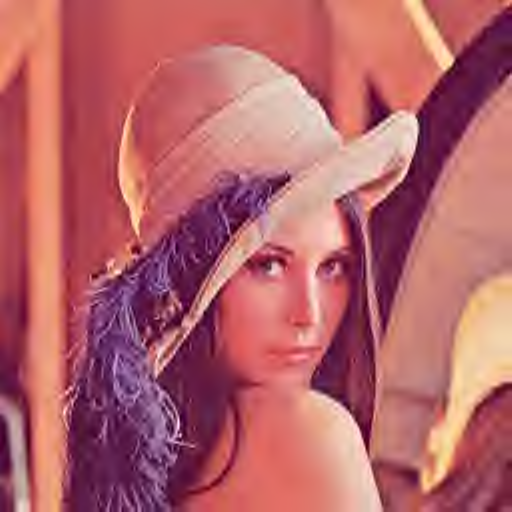
\includegraphics[width=0.45\textwidth]{graphics/lena_01_jp2}\\
  \vspace{-25ex}\hspace{19ex}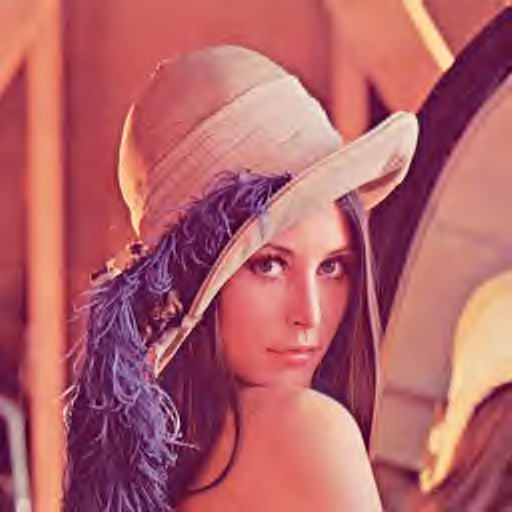
\includegraphics[width=0.45\textwidth]{graphics/lena_02_jp2}\\
  \vspace{-25ex}\hspace{38ex}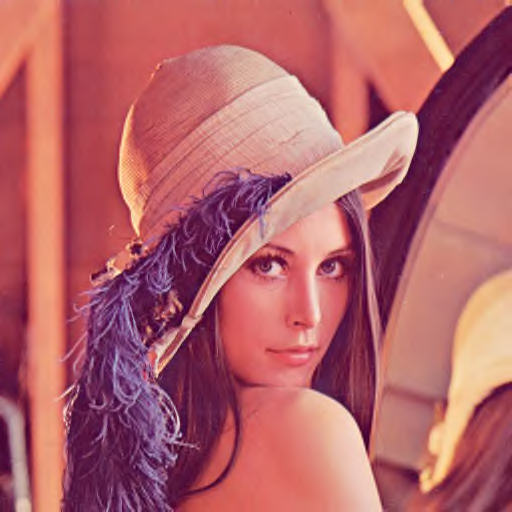
\includegraphics[width=0.45\textwidth]{graphics/lena_05_jp2}
}}
\end{flushleft}
\subsection{Spatial scalabilty}
\begin{itemize}
\item Enables a progressive transmission by resolution (more decoded
  data, more resolution).
\item Ideal for simulcasting.
\end{itemize}
\begin{center}
  \resizebox{0.9\textwidth}{!}{
    \begin{tabular}{ccc}
      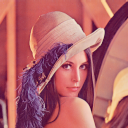
\includegraphics{graphics/lena_128x128_rgb} & 
      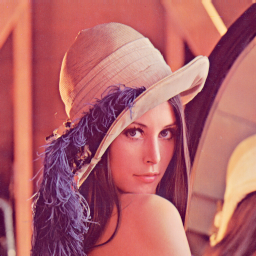
\includegraphics{graphics/lena_256x256_rgb} & 
      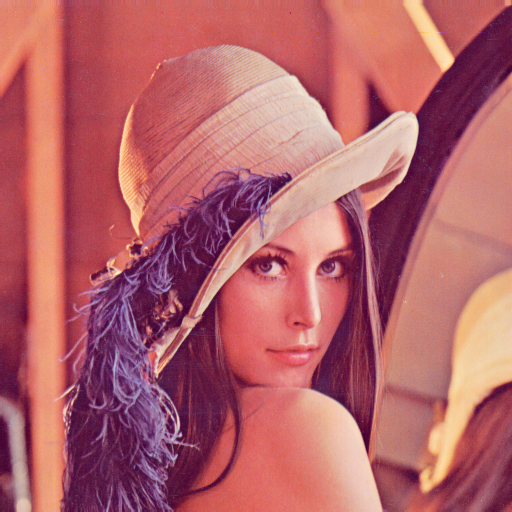
\includegraphics{graphics/lena_512x512_rgb}
    \end{tabular}
  }
\end{center}
\subsection{ROI (Regions Of Interest) scalability}
\begin{center}
  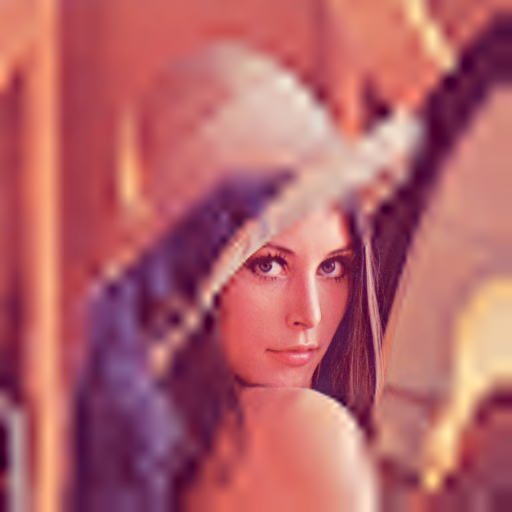
\includegraphics[height=\pagegoal - \pagetotal - 1cm]{graphics/lena_512x512_rgb_jp2_roi}
\end{center}
\end{comment}

\section*{Reduction of the distortion of a coding pass}
\begin{itemize}
\item The contribution to the quality (distortion decrease) of a
  coding pass to the total distortion of the reconstruction is
  determined by:
  \begin{enumerate}
  \item The weight of the bits of the coefficients that are encoded in
    the coding pass.
  \item The energy gain factor of the subband where the code-block is
    located.
  \end{enumerate}
\end{itemize}

\section*{Progressions of JPEG2000}
\begin{itemize}
\item In fact, a JPEG 2000 codec produces a packet for each precinct,
  component, resolution level and quality layer.
\item Depending on the final packet ordering, we have one of the
  following progressions:
\end{itemize}

\section*{LRCP or quality progression}
\begin{itemize}
\item Packets are ordered first by quality, then by resolution level,
  then by component and finally, by precinct. Example:
\end{itemize}
\begin{center}
  \svg{graphics/LRCP}{800}
\end{center}

\section*{RLCP or spatial progression}
\begin{itemize}
\item Packets are ordered first by resolution level, then by quality
  layer, then by component and finally, by precinct. Example:
\end{itemize}
\begin{center}
  \svg{graphics/RLCP}{800}
\end{center}

\section*{PCRL or sequential progression}
\begin{itemize}
\item Packets are ordered first by precinct, then by component, after
  that by spatial resolution and finally, by quality layer. Example:
\end{itemize}
\begin{center}
  \svg{graphics/PCRL}{800}
\end{center}

\section*{Rudimentary ROI definition at decoding time}
\begin{itemize}
\item The random access to the packet-stream give the possibility of
  the definition of a ROI by the decoder.
\item The accuracy of the shape of the ROI depends on the precinct
  size(s). The smaller the precincts, the better the precision.
\item This feature is typically exploited in client/server
  architectures through the JPIP (JPeg 2000 Interactive
  Protocol)~\cite{JPIP}.
\end{itemize}

\section*{``Lena'' at $0.1$ bpp}
\begin{center}
  \begin{tabular}{cc}
    JPEG ($21.29$ dB) & JPEG2000 ($27.03$ dB) \\
    \jpg{graphics/lena_01} &
    \png{graphics/lena_01_jp2}{512}
    % \image{0.45\textwidth}{lena_01_jpg} & \image{0.45\textwidth}{lena_01_jp2}
  \end{tabular}
\end{center}


\section*{``Lena'' at $0.2$ bpp}
\begin{center}
  \begin{tabular}{cc}
    JPEG ($26.64$ dB) & JPEG2000 ($29.22$ dB) \\
    \jpg{graphics/lena_02} &
    \png{graphics/lena_02_jp2}{512}
    % \image{0.45\textwidth}{lena_02_jpg} & \image{0.45\textwidth}{lena_02_jp2}
  \end{tabular}
\end{center}

\section*{``Lena'' at $0.3$ bpp}
\begin{center}
  \begin{tabular}{cc}
    JPEG ($28.97$ dB) & JPEG2000 ($30.71$ dB) \\
    \jpg{graphics/lena_03} &
    \png{graphics/lena_03_jp2}{512}
    % \image{0.45\textwidth}{lena_03_jpg} & \image{0.45\textwidth}{lena_03_jp2}
  \end{tabular}
\end{center}

\section*{``Lena'' at $0.4$ bpp}
\begin{center}
  \begin{tabular}{cc}
    JPEG ($30.09$ dB) & JPEG2000 ($31.58$ dB) \\
    \jpg{graphics/lena_04} &
    \png{graphics/lena_04_jp2}{512}
    % \image{0.45\textwidth}{lena_04_jpg} & \image{0.45\textwidth}{lena_04_jp2}
  \end{tabular}
\end{center}

\section*{``Lena'' at $0.5$ bpp}
\begin{center}
  \begin{tabular}{cc}
    JPEG ($30.91$ dB) & JPEG2000 ($32.24$ dB) \\
    \jpg{graphics/lena_05} &
    \png{graphics/lena_05_jp2}{512}
    % \image{0.45\textwidth}{lena_05_jpg} & \image{0.45\textwidth}{lena_05_jp2}
  \end{tabular}
\end{center}

\section*{``Cat'' at $0.1$ bpp}
\begin{center}
  \begin{tabular}{cc}
    JPEG ($17.79$ dB) & JPEG2000 ($23.33$ dB) \\
    \jpg{graphics/cat_01} &
    \png{graphics/cat_01_jp2}{512}
    % \image{0.5\textwidth}{cat_01_jpg} & \image{0.5\textwidth}{cat_01_jp2}
  \end{tabular}
\end{center}

\section*{``Cat'' at $0.2$ bpp}
\begin{center}
  \begin{tabular}{cc}
    JPEG ($23.59$ dB) & JPEG2000 ($25.97$ dB) \\
    \jpg{graphics/cat_02} &
    \png{graphics/cat_02_jp2}{512}
    % \image{0.5\textwidth}{cat_02_jpg} & \image{0.5\textwidth}{cat_02_jp2}
  \end{tabular}
\end{center}

\section*{``Cat'' at $0.3$ bpp}
\begin{center}
  \begin{tabular}{cc}
    JPEG ($25.63$ dB) & JPEG2000 ($27.60$ dB) \\
    \jpg{graphics/cat_03} &
    \png{graphics/cat_03_jp2}{512}
    % \image{0.5\textwidth}{cat_03_jpg} & \image{0.5\textwidth}{cat_03_jp2}
  \end{tabular}
\end{center}

\section*{``Cat'' at $0.4$ bpp}
\begin{center}
  \begin{tabular}{cc}
    JPEG ($27.10$ dB) & JPEG2000 ($28.97$ dB) \\
    \jpg{graphics/cat_04} &
    \png{graphics/cat_04_jp2}{512}
    % \image{0.5\textwidth}{cat_04_jpg} & \image{0.5\textwidth}{cat_04_jp2}
  \end{tabular}
\end{center}

\section*{``Cat'' at $0.5$ bpp}
\begin{center}
  \begin{tabular}{cc}
    JPEG ($28.23$ dB) & JPEG2000 ($30.08$ dB) \\
    \jpg{graphics/cat_05} &
    \png{graphics/cat_05_jp2}{512}
    % \image{0.5\textwidth}{cat_05_jpg} & \image{0.5\textwidth}{cat_05_jp2}
  \end{tabular}
\end{center}

\section{Motion JPEG 2000}
\begin{itemize}
\item As in JPEG, JPEG 2000 has an extension \cite{j2k-part3} to
  compress sequences of images.
\item Each image is encoded independently.
\item But at difference of JPEG, the code-streams can be variable
  bit-rate (compression ratio selected by slope(s)) or constant
  bit-rate (compression ratio selected by bit-rate(s)).
\item Finally, scalability can be used to recover a reduced quality,
  lower ROI/resolution or gray-scale version of the original image. 
\end{itemize}
\begin{center}
  \svg{graphics/MJ2K_ir}{600}
\end{center}

In the III... (or Intra video) coding, the
\href{https://sistemas-multimedia.github.io/milestones/07-DCT/}{2D
  block-DWT}, the
\href{https://sistemas-multimedia.github.io/milestones/08-DWT/}{2D
  DWT}, or any other spatial transform, is used on sequences of frames
(images) to exploit the spatial correlation. This is achieved by
simply iterating the spatial decorrelation as it is described in the
Algorithm~\ref{alg:III_coding}~\cite{taubman2002jpeg2000}, where $V$
in the input sequence and $S$ controls the number of SRLs (Spatial
Resolution Levels)\footnote{Notice that at least one SRL is always
available for each image or video sequence}. The synthesis transform
is computed using the Algorithm~\ref{alg:III_decoding}. In the
Fig.~\ref{fig:III} there is an example of the decomposition generated
for three frames $V_0$, $V_1$ and $V_2$.

\begin{myalg}{III-coding}{$\mathbf{V}$ /* original video sequence */, $S$ /* Number of extra levels */}{$\mathbf{O}$ /* transformed video sequence */}
  \label{alg:III_coding}
  \begin{enumerate}
  \item ${\mathbf O}=\{\}$ /* empty sequence */.
  \item for ${\mathbf V}_i\in {\mathbf V}$:
    \begin{enumerate}
    \item ${\mathbf O}_i\leftarrow\text{2D-T}^{S}({\mathbf V}_i)$ /* 2D analysis spatial transform */.
    \end{enumerate}
  \end{enumerate}
\end{myalg}

\begin{myalg}{III-decoding}{$\mathbf{O}$ /* transformed video sequence */, $S$ /* Number of extra levels */}{$\mathbf{V}$ /* original video sequence */}
  \label{alg:III_decoding}
  \begin{enumerate}
  \item ${\mathbf V}=\{\}$ /* empty sequence */.
  \item for ${\mathbf O}_i\in {\mathbf O}$:
    \begin{enumerate}
    \item ${\mathbf V}_i\leftarrow\text{2D-T}^{-S}({\mathbf O}_i)$ /* 2D synthesis spatial transform */.
    \end{enumerate}
  \end{enumerate}
\end{myalg}

\begin{figure}
  \centering
  \myfig{graphics/forward_MDWT}{6cm}{600}
  \caption{Decomposition generated by 1-levels ($S=1$) 2D-DWT and the 2x2-DCT (block size is equal to $S+1$).}
  \label{fig:III}
\end{figure}

\section*{Lab}
\begin{itemize}
\item Download and compile the Kakadu software implementation for the
  JPEG 2000 standard.
\item Find the R/D curve for the image lena using one quality layer
  (re-do the same experiment that in JPEG: compress and expand
  the image for several bit-rates and compute the RMSE). Use both, the
  reversible and the irreversible paths.
\item Now, let's take advantage of the scalability of JPEG 2000!
  Compress lena without loss (using the reversible path) and one
  quality layer, and find the R/D curve truncating the
  code-stream. Re-do the experiment for different quality
  layers. Which alternative is best?
\end{itemize}

% \newpage
% \section[~Compresi'on de ``akiyo'']{Compresi'on de ``akiyo'' }
% \begin{itemize}
% \item Al igual que JPEG, JPEG2000 no puede comprimir secuencias de
%   im'agenes, pero puede ser llamado iterativamente para generar un
%   resultado semejante (M-JPEG2000). La ventaja de JPEG2000 radica en
%   que adem'as de alcanzar mejores tasas de compresi'on, podemos
%   conseguir que cada imagen tenga el n'umero de bits deseados.
% \item Para comprimir ``akiyo'', utilizaremos una versi'on comercial del
%   est'andar JPEG2000 llamada Kakadu
%   (\texttt{http://www.kakadusoftware.com}). Al igual que con JPEG,
%   usaremos una tasa de compresi'on de $25$ (o $0.96$ bits/pixel). El
%   comando usado para comprimir la secuencia ha sido:
% \newpage
% \begin{verbatim}
% for i in akiyo???
% do
%   kdu_compress -i $i -o $i.jp2 -rate 0.96
% done 
% \end{verbatim} %$
% \item De forma semejante a M-JPEG, M-JPEG2000 permite la
%   escalabilidad temporal. Sin embargo, tambi'en disponemos del resto de
%   escalabilidades: espacial, en calidad y ROI.
% \item Kakadu tambi'en dispone de una utilidad para comprimir
%   directamente ficheros YUV usando M-JPEG2000. V'ease el Ap'endice
%   \ref{ape:vids_make} para ver el comando de llamada a esta utilidad.
% \item En el directorio \texttt{vids} encontrar'a diferentes secuencias
%   de v'ideo codificadas con M-JPEG2000. Busque los ficheros
%   \texttt{*MJEG2000*}.
% \end{itemize}

%%% Local Variables: 
%%% mode: latex
%%% TeX-master: t
%%% End: 

\bibliography{JPEG2000}
